%!TEX TS-program = xelatex
%!TEX encoding = UTF-8 Unicode
%!TEX root = 2020-GS-ARTICLE.tex
%-------------------------------------------------------------------------------
%-------------------------------------------------------------------------------
%	PACKAGES AND OTHER DOCUMENT CONFIGURATIONS
%-------------------------------------------------------------------------------
%-------------------------------------------------------------------------------
\documentclass[
	a4paper,
	twocolumn
	]{article}
%--------------------------------------------------------------- GENERAL SETUP -
\usepackage[T1]{fontenc}
\usepackage[italian]{babel}
\usepackage{
  graphicx,
  dblfloatfix
}
\usepackage{graphicx}
\usepackage{epstopdf}
\epstopdfsetup{update}
\usepackage[usenames]{color}
\usepackage{amssymb}
\usepackage{hyperref} % For hyperlinks in the PDF
%---------------------------------------------------------------- STYLE GS2020 -
%-------------------------------------------------------------------------------
%-------------------------------------------------------------------------------
%	CUSTOM PACKAGES AND OTHER DOCUMENT CONFIGURATIONS
%-------------------------------------------------------------------------------
%-------------------------------------------------------------------------------
\usepackage{Alegreya}
\linespread{1.05}
\usepackage{
	fontspec,
	xltxtra,
	xunicode
	}

\usepackage{
	xfrac,
	unicode-math
	}

\defaultfontfeatures{Mapping=tex-text}
\setmonofont[
	Scale=MatchLowercase
	]{Andale Mono}
\setmathfont[
	Scale=MatchLowercase,
	Scale=1
	]{Libertinus Math}

\usepackage{microtype}
\usepackage[
	top=20mm,
	bottom=25mm,
	textwidth=17.2cm,
	columnsep=0.8cm
	]{geometry}
\usepackage[
	hang,
	small,
	labelfont=bf,
	up,
	textfont=it,
	up
	]{caption}
\usepackage{paralist} % For compact item lists
\usepackage{etoolbox} % Some tools: used for quote environment
\AtBeginEnvironment{quote}{\small}
\usepackage{titling} % Customizing the title section
\usepackage{booktabs} % Horizontal rules in tables
\usepackage{enumitem} % Customized lists
\setlist[itemize]{noitemsep} % Make itemize lists more compact
\usepackage{abstract} % Allows abstract customization
\renewcommand{\abstractnamefont}{\normalfont\bfseries} % Set the "Abstract" text to bold
\renewcommand{\abstracttextfont}{\normalfont\small\itshape} % Set the abstract itself to small italic text
\usepackage{titlesec} % Allows customization of titles
\renewcommand\thesection{\Roman{section}} % Roman numerals for the sections
\renewcommand\thesubsection{\Roman{subsection}} % roman numerals for subsections
\titleformat{\section}[block]{\large\centering}{\thesection.}{1em}{} % Change the look of the section titles
\titleformat{\subsection}[block]{\large}{\thesubsection.}{1em}{} % Change the look of the section titles
%-------------------------------------------------------------------------------
%-------------------------------------------------------------------------------
%	TITLE SECTION
%-------------------------------------------------------------------------------
%-------------------------------------------------------------------------------
\setlength{\droptitle}{-4\baselineskip} % Move the title up
\pretitle{\begin{center}\huge\bfseries} % Article title formatting
\posttitle{\end{center}} % Article title closing formatting
\title{Superstereo Synth \\ \large{\emph{Relazione STALPM}}} % Article title
\author{%
\textsc{Giuseppe Messineo}\\%[1ex]%
\normalsize Conservatorio G. Nicolini Piacenza \\ % Your institution
\normalsize giuseppe.messineo@conservatorio.piacenza.it % Your email address
%\and % Uncomment if 2 authors are required, duplicate these 4 lines if more
%\textsc{Wikio Orgopedio}\\%[1ex]%
%\normalsize Conservatorio S. Cecilia di Roma \\ % Your institution
%\normalsize wikio @ orgopedio.com % Your email address
}
\date{} % Leave empty to omit a date

\usepackage{fancyhdr} % Headers and footers
\pagestyle{fancy} % All pages have headers and footers
\fancyhead{} % Blank out the default header
\fancyfoot{} % Blank out the default footer
\fancyhead[C]{\small STALPM 1 • Relazione} % Custom header text
\fancyfoot[RO,LE]{\small \today~ • w: \input{includes/words.txt} • c: \input{includes/char.txt} • p:~\thepage} % Custom footer text
%-------------------------------------------------------------------------------
%-------------------------------------------------------------------------------
%	LISTINGS
%-------------------------------------------------------------------------------
%-------------------------------------------------------------------------------
\usepackage{listings}
% lstlistings setup
\definecolor{yobg}{rgb}{0.9,0.9,1}
\definecolor{yotxt}{rgb}{0.01,0.01,0.52} % a dark blue.
\definecolor{mylstbg}{rgb}{0.98,0.98,0.98} % a really pale grey.
\definecolor{mylstcmt}{rgb}{0.01,0.52,0.01} % a dark green.
\definecolor{mylstdoc}{rgb}{0.80,0.30,0.80} % a medium pink.

\lstset{%
  aboveskip=10pt,
	belowskip=5pt,
  language=C++,
  numbers=none,%left,%none,
  tabsize=4,
  %frame=single,
  breaklines=true,
  numberstyle=\tiny\ttfamily,
  backgroundcolor=\color{mylstbg},
  basicstyle=\footnotesize\ttfamily,
  commentstyle=\slshape\color{mylstcmt}, %\itshape,
  %frameround=tttt,
  columns=flexible, %fixed,
  showstringspaces=false,
  emptylines=2,
  inputencoding=utf8,
  extendedchars=true,
  literate=	{á}{{\'a}}1
			{à}{{\`a}}1
			{ä}{{\"a}}1
			{â}{{\^a}}1
			{é}{{\'e}}1
			{è}{{\`e}}1
			{ë}{{\"e}}1
			{ê}{{\^e}}1
			{ï}{{\"i}}1
			{î}{{\^i}}1
			{ö}{{\"o}}1
			{ô}{{\^o}}1
			{è}{{\`e}}1
			{ù}{{\`u}}1
			{û}{{\^u}}1
			{ç}{{\c{c}}}1
			{Ç}{{\c{C}}}1,
  emph={component, declare, environment, import, library, process},
  emph={[2]ffunction, fconstant, fvariable},
  emph={[3]button, checkbox, vslider, hslider, nentry, vgroup, hgroup, tgroup, vbargraph, hbargraph, attach},
  emphstyle=\color{yotxt}, %\underline, %\bfseries,
  morecomment=[s][\color{mylstdoc}]{<mdoc>}{</mdoc>},
  rulecolor=\color{black}
}

%-------------------------------------------------------------------- ABSTRACT -
\renewcommand{\maketitlehookd}{%
\begin{abstract}
\noindent\input{includes/abstract.txt}
\end{abstract}
}
%-------------------------------------------------------------------------------
%-------------------------------------------------------------------------------
%	BEGIN DOCUMENT
%-------------------------------------------------------------------------------
%-------------------------------------------------------------------------------
\begin{document}
\maketitle
\thispagestyle{empty}
%-------------------------------------------------------------------------------
%-------------------------------------------------------------------------------
\section*{INTRODUZIONE}
Partendo dal presupposto che la finalità del corso di STALPM 1 fosse quella
di costruire un oggetto multimimediale indirizzato al web e che quindi se ne
potesse usufruire anche in modo "non-locale", si è ragionato fin dalle prime
lezioni sulla tipologia dell'oggetto in questione. Abbiamo quindi effettuato
un veloce brainstorming sicchè la realizzazione dell'oggetto multimediale
potesse sia portarci ad una finalità pratica, cioè quella di potere utilizzare
esso come un nostro strumento di composizione, sia di apprendimento dei concetti
basilari del mondo della programmazione, a noi sconosciuto o quasi fino a quel
momento. Il frutto dei nostri ragionamenti è stato quello di realizzare un synth,
inizialmente con l'idea di basarci su di un modello presistente, poi quella di
realizzarne un modello con una struttura dei vari moduli e percorso del segnale
nuova, rispetto a quelle che erano i nostri pensieri al momento della decisione.
Per la realizzazione dello "Superstereo Synth" si è subito pensato a quale fosse
la strada più efficace da intraprendere per la realizzazione del nostro
sintetizzatore, partendo come detto da una conoscenza quasi nulla rispetto al
mondo della programmazione.  a che tipo di
sintetizzatore realizzare, ponendoci fin da subito la questione
%-------------------------------------------------------------------------------
\subsubsection*{DESCRIZIONE DEL CODICE}
La parte iniziale del codice denominata “GUI” contiene tutti i gruppi grafici dentro i quali abbiamo inserito i vari elementi –grafici appunto- del nostro strumento di sintesi quali knob, fader, pulsanti e meter.

%-----------------------------------------------------
%-------------------------larghezza massima del codice
\begin{lstlisting}
// GUI
main(x) = hgroup("[01] Superstereo Synth",x);
s_g(x) = main(vgroup("[01] SUBTRACTIVE",x));
m_g(x) = main(vgroup("[03] MASTER",x));
p_g(x) = main(vgroup("[05] PHASER",x));
lmeter(x) = main(attach(
	x,an.amp_follower(0.150,x) : ba.linear2db :
	vbargraph("[02] L [unit:dB]", -70,0)));
rmeter(x) = main(attach(
	x,an.amp_follower(0.150,x) : ba.linear2db :
	vbargraph("[04] R [unit:dB]", -70,0)));
meters = lmeter, rmeter;
\end{lstlisting}

Il modulo di sintesi sottrattiva chiamato “SUBTRACTIVE” contiene al suo interno un generatore di rumore bianco e uno di dente di sega con frequenza fissa, swichabili tramite un apposito pulsante. Il tutto va dentro un filtro risonante “Ladder” basato sul modello di Robert Moog con relativi controlli di f cut e Q factor, ed in seguito ad un cotrollo di ampiezza.
Il modulo di sottrattiva è posto nella parte destra del synth.


%-----------------------------------------------------
%-------------------------larghezza massima del codice
\begin{lstlisting}
// SUBTRACTIVE
// Sawfreq Custom
sawfreq = 123;
generator = (no.noise *switch),
	(os.sawtooth(sawfreq)*(1-switch)) :> _;
switch = s_g(checkbox("[01] Saw/Noise")) : si.smoo;
gain = s_g(
	vslider("[04] Gain [style:knob]",-12,-96,+12,0.01))
	: ba.db2linear : si.smoo;
Q = s_g(
	vslider("[03] Q [style:knob]",5,0.7072,25,0.01));
fcut = s_g(
	vslider("[02] Cut [style:knob]",0.65,0,1,0.001)) :
	si.smoo;
subtractive = generator : ve.moogLadder(fcut,Q) :
	*(gain);
\end{lstlisting}


Di seguito troviamo un Phaser Stereo chiamato “PHASERSYNTH”, costruito tramite una sequenza di N allpass, come dal modello di Curtis Roads su “The Computer Music Tutorial”, di cui il canale R agisce di fase opposta al canale L. Il segnale verrà reso stereofonico tramite la tecnica dello “Stereo Shuffling”. Lo “Superstereophaser” (così chiamato citando il film “Ritorno al futuro”), avrà 3 tipi di controlli tramite dei knob:
\begin{compactitem}
\item LFO frequency
\item Feedback
\item Delay
\end{compactitem}

%-----------------------------------------------------
%-------------------------larghezza massima del codice
\begin{lstlisting}
// PHASER
lff = p_g(
	vslider("[02] Lfo [style:knob]",0.358, 0, 16, 0.001))
	: si.smoo;
fbk = p_g(
	vslider("[03] Feedback [style:knob]",
	        -0.689, -0.999, 0.999, 0.001) : si.smoo);
del = p_g(
	nentry("[04] Delay [style:knob]",1, 1, 100, 1));

lfo = os.osc(lff);

phaserLR(N,x,d,g,fb) = x <: l,r
with{
  allpassL(d,g) = (+ <: de.fdelay(
		(ma.SR/2),d),*(-g)) ~ *(g) : mem,_ : +;
  allpassR(d,g) = (+ <: de.fdelay(
		(ma.SR/2),d),*(g)) ~ *(-g) : mem,_ : +;
  apseqL(N,d,g) = seq(i,N,allpassL(d,g));
  apseqR(N,d,g) = seq(i,N,allpassR(d,g));

  l= _, (+:apseqL(N,d,g))~*(fb):> _;
  r=  _, (+:apseqR(N,d,g))~*(-fb):> _;
};

// STEREO SHUFFLER
pot = m_g(
	vslider("[02] WIDE [style:knob]",100,0,200,0.1)) :
	/(100) : si.smoo;
somma = + : /(2);
diff = - : /(2);
sdm = somma,diff;
wide = _, * (sqrt(pot));
stereoshuffle= _,_ <: sdm : wide <: sdm;

superstereophaser = phaserLR(4,_,del,lfo,fbk) :
	stereoshuffle;
\end{lstlisting}
%-----------------------------------------------------
%-------------------------larghezza massima del codice

Lo “Superstereophaser” è posto sulla parte destra del synth e potrà essere bypassato tramite un apposito pulsante posto in cima alla sezione stessa.
Successivamente, il nostro segnale entrerà all’interno di un numero N di chopper (Hard Limiter) che limiteranno il segnale in modo netto secondo una soglia prestabilita, seguiti da N filtri passa basso di diverso ordine, in modo da rendere più “smooth” il segnale generato, attenuando le armoniche superiori generate dai chopper e mantenere quelle inferiori.

\begin{lstlisting}
// HARD LIMITER
chopper(a) = min(a) : max(-a);

hardlimiter = chopper(0.7) :
	fi.lowpass(12,15000): chopper(0.9) :
	fi.lowpass6e(20000);
phchop = superstereophaser :
	hardlimiter, hardlimiter;
 \end{lstlisting}

Il tutto entrerà nella sezione chiamata “MASTER CONTROLS” nella quale avremo in ordine:
- Pulsante “MUTE”, che chiude il segnale alla fine della catena (pre-fader)
- Controllo del volume Master tramite un fader verticale con valori in scala logaritmica posto al centro del synth.
-Due Meters, sempre su scala logaritmica, posti al due lati della sezione Master.
La sezione Master si trova nella parte centrale del nostro Synth.

%-----------------------------------------------------
%-------------------------larghezza massima del codice
\begin{lstlisting}
// MASTER CONTROLS
mute = m_g(*(1-(checkbox("[04] Mute")))) : si.smoo;
volume = m_g(vslider("[02] VOLUME ",-6,-70,12,0.1)) :
   ba.db2linear : si.smoo;
bpc = p_g(checkbox("[01] Bypass"));
phaser = ba.bypass1to2(bpc,phchop);
mutes = mute,mute;
master = (*(volume), *(volume));
\end{lstlisting}

Di seguito la struttura generale del programma, sia in forma di codice che
rappresentata attraverso un diagramma a blocchi (fig.1):

\begin{lstlisting}
process = subtractive : phaser : master : mutes : meters;
\end{lstlisting}

\begin{figure}[h]
\begin{center}
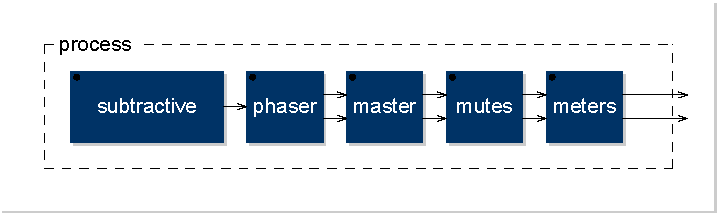
\includegraphics[width=.47\textwidth]{img/process}
\caption{\textbf{Process}. Diagramma a blocchi della struttura del synth.}
\label{gr01}
\end{center}
\end{figure}


%-------------------------------------------------------------------------------
\subsubsection*{UNNUMBERED SUB-SUB-SECTION}
Some predictions of general relativity differ significantly from those of
classical physics, especially concerning the passage of time, the geometry of
space, the motion of bodies in free fall, and the propagation of light. Examples
of such differences include gravitational time dilation, gravitational lensing,
the gravitational redshift of light, and the gravitational time delay. The
predictions of general relativity in relation to classical physics have been
confirmed in all observations and experiments to date. Although general
relativity is not the only relativistic theory of gravity, it is the simplest
theory that is consistent with experimental data. However, unanswered questions
remain, the most fundamental being how general relativity can be reconciled with
the laws of quantum physics to produce a complete and self-consistent theory of
quantum gravity.

Einstein's theory has important astrophysical implications. For example, it
implies the existence of black holes regions of space in which space and time
are distorted in such a way that nothing, not even light, can escape as an
end state for massive stars. There is ample evidence that the intense radiation
emitted by certain kinds of astronomical objects is due to black holes. For
example, microquasars and active galactic nuclei result from the presence of
stellar black holes and supermassive black holes\ldots


\vfill\null

\begin{figure}[b]
\begin{center}
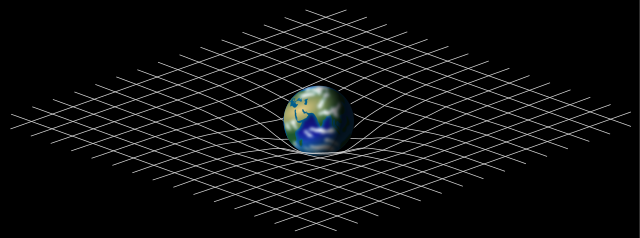
\includegraphics[width=.47\textwidth]{img/image1.png}
\caption{\textbf{Spacetime curvature schematic}. Lattice analogy of the deformation
of spacetime caused by a planetary mass.}
\label{gr01}
\end{center}
\end{figure}

\newpage % USE NEWPAGE TO FORCE COLUMNN INTERRUPTION
%-------------------------------------------------------------------------------
%-------------------------------------------------------------------------------
\section*{UNNUMBERED SECTION}

\begin{quote}
La musica non e` solo composizione. \\
Non è artigianato, non è un mestiere. \\
La musica è pensiero.\cite{nono85}.
\end{quote}

Some predictions of general relativity differ significantly from those of
classical physics, especially concerning the passage of time, the geometry of
space, the motion of bodies in free fall, and the propagation of light. Examples
of such differences include gravitational time dilation, gravitational lensing,
the gravitational redshift of light, and the gravitational time delay. The
predictions of general relativity in relation to classical physics have been
confirmed in all observations and experiments to date. Although general
relativity is not the only relativistic theory of gravity, it is the simplest
theory that is consistent with experimental data. However, unanswered questions
remain, the most fundamental being how general relativity can be reconciled with
the laws of quantum physics to produce a complete and self-consistent theory of
quantum gravity.

\begin{table}[htp]
\begin{center}
\begin{tabular}{ll}
\textbf{Stages} & \textbf{Dur.} \\
\hline
\textbf{Omnidirectional Expositions} & 6 mo. \\
Sound-shape analysis and visualizations & \\
Sound-shape reproduction & \\
Sound-shape database design & \\
\hline
\textbf{Micro-Rhythm of sound-shape} & 12 mo. \\
Solo repertoire analysis & \\
Sound-shape explosion in practising & \\
From literature to shapes open-data & \\
\hline
\textbf{Rhythm of sound-shape interactions} & 12 mo. \\
Multiple sources multiple shapes & \\
Relationship and complexity perception & \\
\hline
\textbf{Sound-shape in musical composition} & 12 mo. \\
AI: unleashed writing opportunities & \\
AI: can you listen the time? & \\
\hline
\textbf{Final documentation} & 6 mo. \\
\end{tabular}
\label{timesheet}
\caption{Thinking Tetrahedral Today stages}
\end{center}
\end{table}%

Einstein's theory has important astrophysical implications. For example, it
implies the existence of black holes regions of space in which space and time
are distorted in such a way that nothing, not even light, can escape as an
end state for massive stars. There is ample evidence that the intense radiation
emitted by certain kinds of astronomical objects is due to black holes. For
example, microquasars and active galactic nuclei result from the presence of
stellar black holes and supermassive black holes, respectively. The bending of
light by gravity can lead to the phenomenon of gravitational lensing, in which
multiple images of the same distant astronomical object are visible in the sky.
General relativity also predicts the existence of gravitational waves, which
have since been observed directly by the physics collaboration LIGO. In addition,
general relativity is the basis of current cosmological models of a consistently
expanding universe.

\begin{compactitem}
\item Derivations of the Lorentz transformations
\item Einstein–Hilbert action
\item Tests of general relativity
\item Two-body problem in general relativity
\end{compactitem}

\begin{figure}[t]
\centering
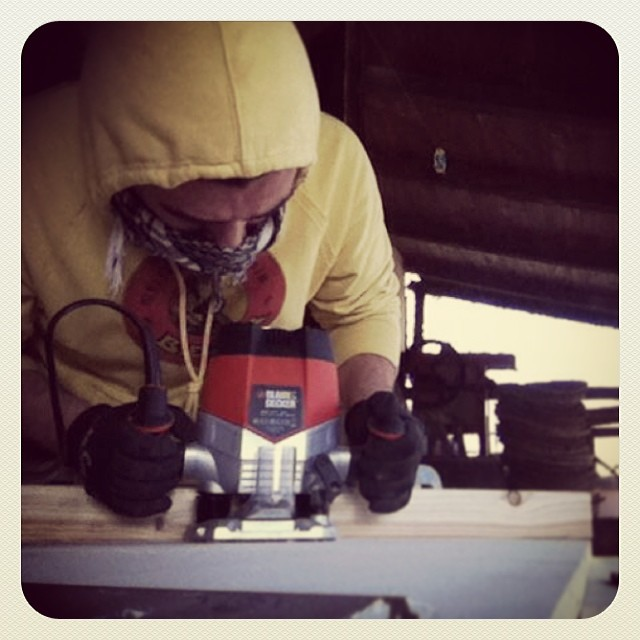
\includegraphics[width=.47\textwidth]{img/image2.jpg}
\caption{Mind Mapping}
\label{gs}
\end{figure}

\begin{equation}
m(x,p,\theta) = (p*x) + ((1-p)*(x\cos\theta)
\label{eq:mid}
\end{equation}

Some predictions of general relativity differ significantly from those of
classical physics, especially concerning the passage of time, the geometry of
space, the motion of bodies in free fall, and the propagation of light.

%--------------------------------------------
%----------------larghezza massima del codice
\begin{lstlisting}
mspan(x,p,rad) = m,s
with{
  m = (p*x)+((1-p)*(x*cos(rad)));
  s = x*(sin(-rad));
};
\end{lstlisting}

Examples
of such differences include gravitational time dilation, gravitational lensing,
the gravitational redshift of light, and the gravitational time delay. The
predictions of general relativity in relation to classical physics have been
confirmed in all observations and experiments to date. Although general
relativity is not the only relativistic theory of gravity, it is the simplest
theory that is consistent with experimental data.

\vfill\null

\raggedright
\bibliographystyle{plain}
\bibliography{includes/bibliography.bib}

\end{document}

%%%%%%%%%%%%%%%%%%%%%%%%%%%%%%%%%%%%%%%%%%%%%%%%%%%%%%%%%%%%%%%%%%%%%%%%%%%%%%%%
% 2020 GIUSEPPE SILVI ARTICLE TEMPLATE BASED ON
%%%%%%%%%%%%%%%%%%%%%%%%%%%%%%%%%%%%%%%%%%%%%%%%%%%%%%%%%%%%%%%%%%%%%%%%%%%%%%%%
% Journal Article
% LaTeX Template
% Version 1.4 (15/5/16)
% This template has been downloaded from:
% http://www.LaTeXTemplates.com
% Original author:
% Frits Wenneker (http://www.howtotex.com) with extensive modifications by
% Vel (vel@LaTeXTemplates.com)
% License:
% CC BY-NC-SA 3.0 (http://creativecommons.org/licenses/by-nc-sa/3.0/)
%%%%%%%%%%%%%%%%%%%%%%%%%%%%%%%%%%%%%%%%%%%%%%%%%%%%%%%%%%%%%%%%%%%%%%%%%%%%%%%%
